\chapter{Bilder}
\section{Bild mit Caption drunter}

Auf dem Bild \ref{fig:featuremap} ist eine Feature Map zu sehen

\begin{figure}[h]
  \centering
  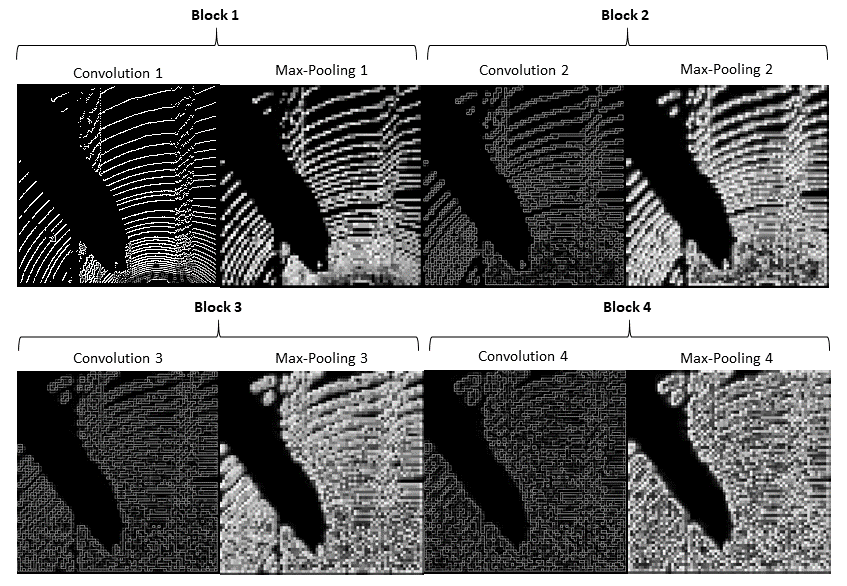
\includegraphics[width=\columnwidth]{img/feature_map.png}
  \caption{Illustration of the extraction of features from a 2D image consisting of LiDAR points, by means of a CNN.} \label{fig:featuremap}
\end{figure}


\section{Zwei Bilder nebeneinander}

Auf der Abbildung \ref{fig:fake_real_objects_examples} sind zwei Bilder zu sehen.

\begin{figure}
  \centering
  \subfigure[Real object with clear shadow]{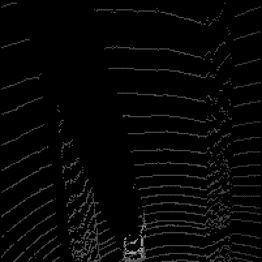
\includegraphics[width=0.45\textwidth]{img/shadowregion.png}}
  \subfigure[Spoofed Object without shadow]{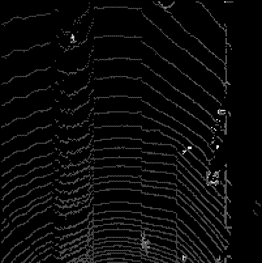
\includegraphics[width=0.45\textwidth]{img/spoofedregion.png}}
  \caption{Result of the 2D image generation, on the one hand with a true object (a) and on the other hand with a spoofed object (b).}
  \label{fig:fake_real_objects_examples} 
\end{figure}

\section{Drei Bilder nebeneinander}

Auf der Abbildung \ref{fig:dreibilder} sind drei Bilder zu sehen.

\begin{figure}[htbp]
    \subfigure[Ressourcen Allokation via Reinforcement Learning] {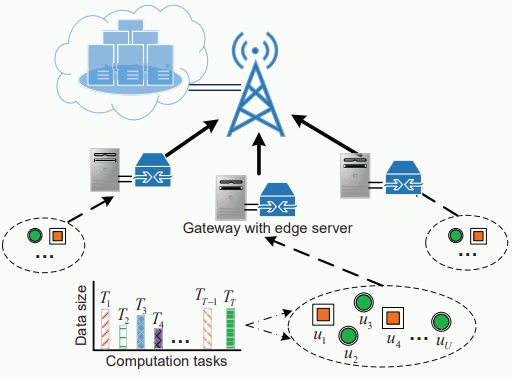
\includegraphics[width=0.33\textwidth]{jointtask07.PNG}}
    \subfigure[Erweitert mit verschiedenen Übertragungsmöglichkeiten] {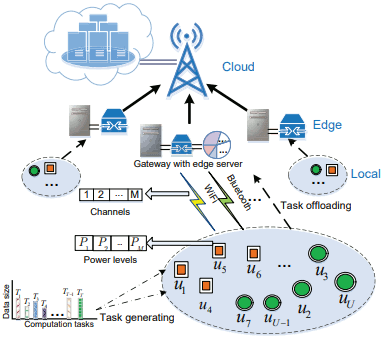
\includegraphics[width=0.33\textwidth]{jointtask05.PNG}} 
    \subfigure[Erweitert durch zentralisierten Clustering-Algorithmus] {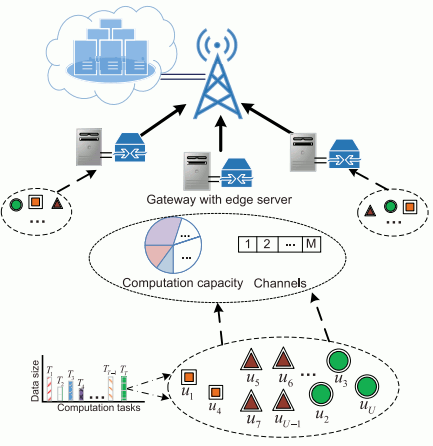
\includegraphics[width=0.33\textwidth]{jointtask08.PNG}}
\caption{Verschiedene Ressourcenallokierungsansätze} 
\label{fig:dreibilder}
\end{figure}

